\section{项目的主要内容和技术路线}

\subsection{主要研究内容}

\par 本研究主要开展如下内容:
\begin{itemize}
  \item [(1)] 数据收集与预处理。
  \par 通过在线开放平台获取2000年-2012年全国县级主要作物产量以及主要作物物候数据集。同时通过NASA官方网站获取MOD17A2、MOD11A2、MOD16A2以及MOD15A2等遥感产品,并利用云计算平台Google Earth Engine进行数据预处理。
  \item [(2)] 估产因子提取。
  \par 通过阅读已有文献并结合自身实验,筛选能有效反应作物生长发育的遥感影像指标作为作物估产因子。
  \item [(3)] 模型构建与训练。
  \par 以中国东北地区为研究区域,选择玉米作为研究作物,以上述估产因子为输入,通过提取遥感影像中时空信息特征获取作物生长信息,并结合往年地区统计的作物产量数据,构建以卷积长短期记忆网络为基础的县域玉米估产模型。
  \item [(4)] 估产模型评价与分析
  \par 将已有的其它模型应用于同一数据集进行县域产量估算,以实际产量统计数据为参考,通过计算不同模型对应的评价指标值,分析对比模型的精度和稳定性。
  \item [(5)] 估产结果分析与评价
  \par 将估产模型应用于其它研究区域或时间段,分析估产结果的时空误差,以及估产结果的时空预测不确定性。
\end{itemize}

\subsection{技术路线}
\begin{itemize}
  \item [(1)] 对2000年-2012年全国县级主要作物产量、主要作物物候数据集和MODIS影像产品进行预处理,以Google Earth Engine为云计算平台,通过编写脚本进行数据清洗,获得东北三省县域玉米年产量以及东北三省历年多光谱影像。
  \item [(2)] 对研究区中的玉米作物进行生长发育期特征分析,以及多源因子和玉米产量的相关性分析,对作物估产模型的输入变量进行选择。
  \item [(3)] 将多元估产因子和历年玉米产量数据作为两个独立编码器(Encoder),通过融合模型(Fusion Module)组合编码器输出特征以提升模型预测精度,最终将融合特征输入解码器(Decoder)进行单步玉米产量预测。
  \item [(4)] 通过测试集测试对比不同模型的评价指标值,分析模型的精度和稳定性。
  \item [(5)] 将估产模型应用于其它研究区域或时间段,进行时空误差分析及时空预测不确定性分析。
\end{itemize}

\begin{figure}
  \begin{center}
    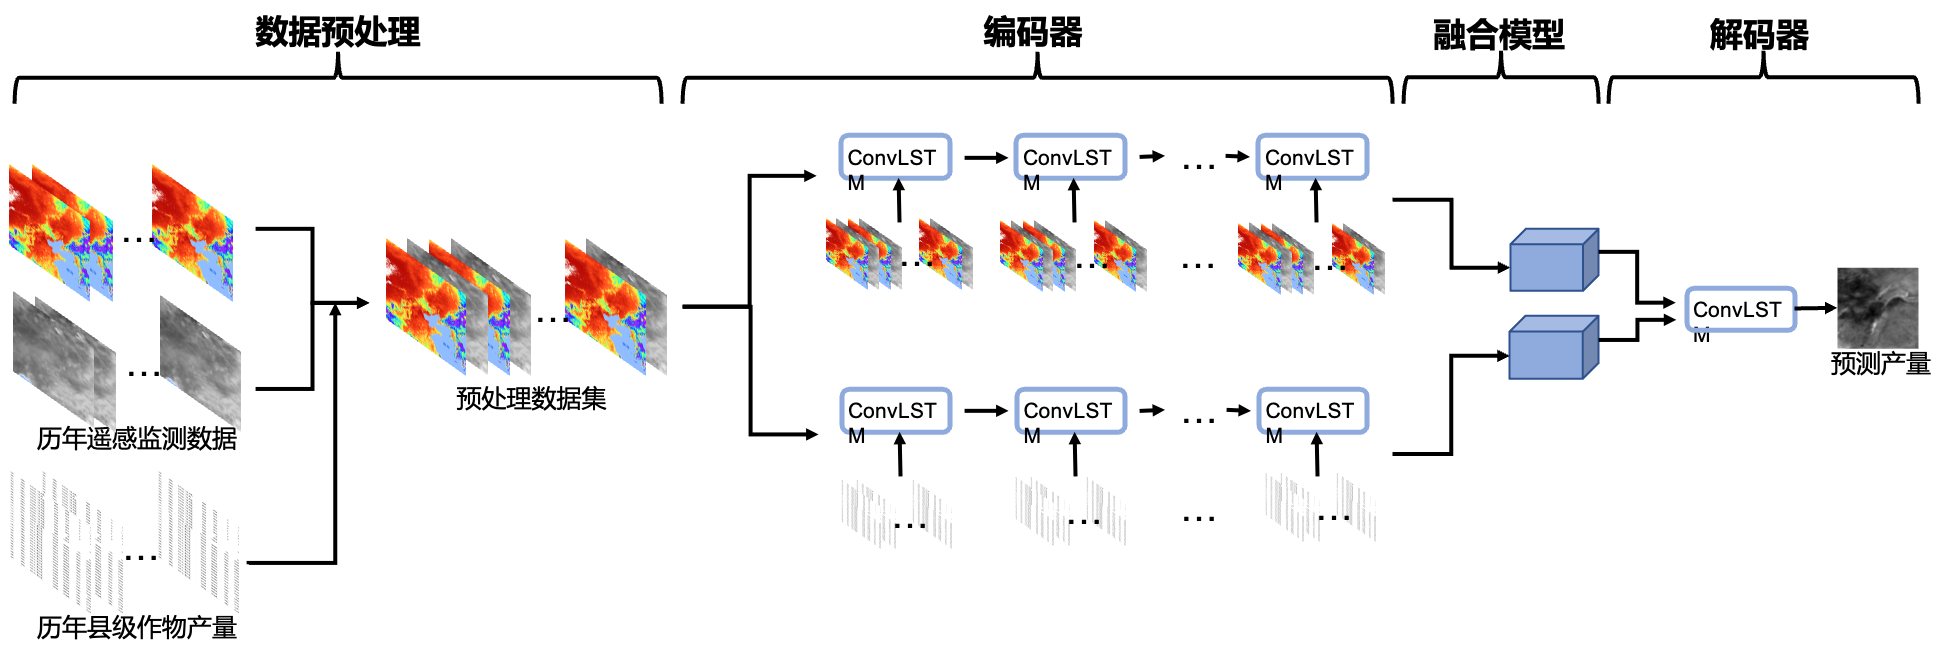
\includegraphics[width=0.8\linewidth]{path.png}
    \caption{技术路线图}
    \label{Fig_path}
  \end{center}
\end{figure}

\subsection{可行性分析}
\begin{itemize}
  \item [(1)] 数据可行性
  \par 研究数据包含了2000年至2012年的县域玉米历年产量、全国2000年至2015年三种主要作物(水稻、小麦、玉米)物候数据集ChinaCropPhen1km,以及研究地区分辨率为1千米的MODIS影像数据,可从NASA官网获取,满足县级玉米估产模型的数据需求。
  \item [(2)] 方法可行性
  \par 已有研究验证了长短期记忆网络能从时序数据挖掘时间关系,能够提取作物生长的多时空遥感观测数据之间的相互关系,相比于循环神经网络,长短期记忆网络在序列问题方面很有效地避免了梯度消失问题。而卷积长短期记忆网络将全联接操作改为了卷积运算,能够从空间数据中有效提取特征。同时,如总初级生产力、表面温度、表面蒸发量、叶面积指数等遥感影像数据已被证明与农作物产量有密切关系。因此,基于多源数据的卷积长短期记忆网络构建县域玉米估产模型具备较高可行性。
  \item [(3)] 硬件可行性
  \par 实验室提供搭载TITAN XP及GeForce RTX 3090 GPU的计算机,满足实验所需的硬件条件。同时,由于遥感影像数据量较大,可以使用云计算平台Google Earth Engine进行处理,实现大规模数据的并行处理,提高计算效率。
\end{itemize}